\documentclass[border=10pt]{standalone}
\usepackage[T1]{fontenc}
\usepackage{amsmath, amssymb}
\usepackage{tikz}
\usetikzlibrary{arrows.meta, positioning, decorations.pathreplacing, calc}

%% Colours
\definecolor{calmblue}{RGB}{41, 98, 255}
\definecolor{panicred}{RGB}{211, 47, 47}
\definecolor{calmfill}{RGB}{227, 236, 255}
\definecolor{panicfill}{RGB}{255, 228, 225}
\definecolor{seqcalm}{RGB}{197, 216, 255}
\definecolor{seqpanic}{RGB}{255, 199, 190}

\begin{document}
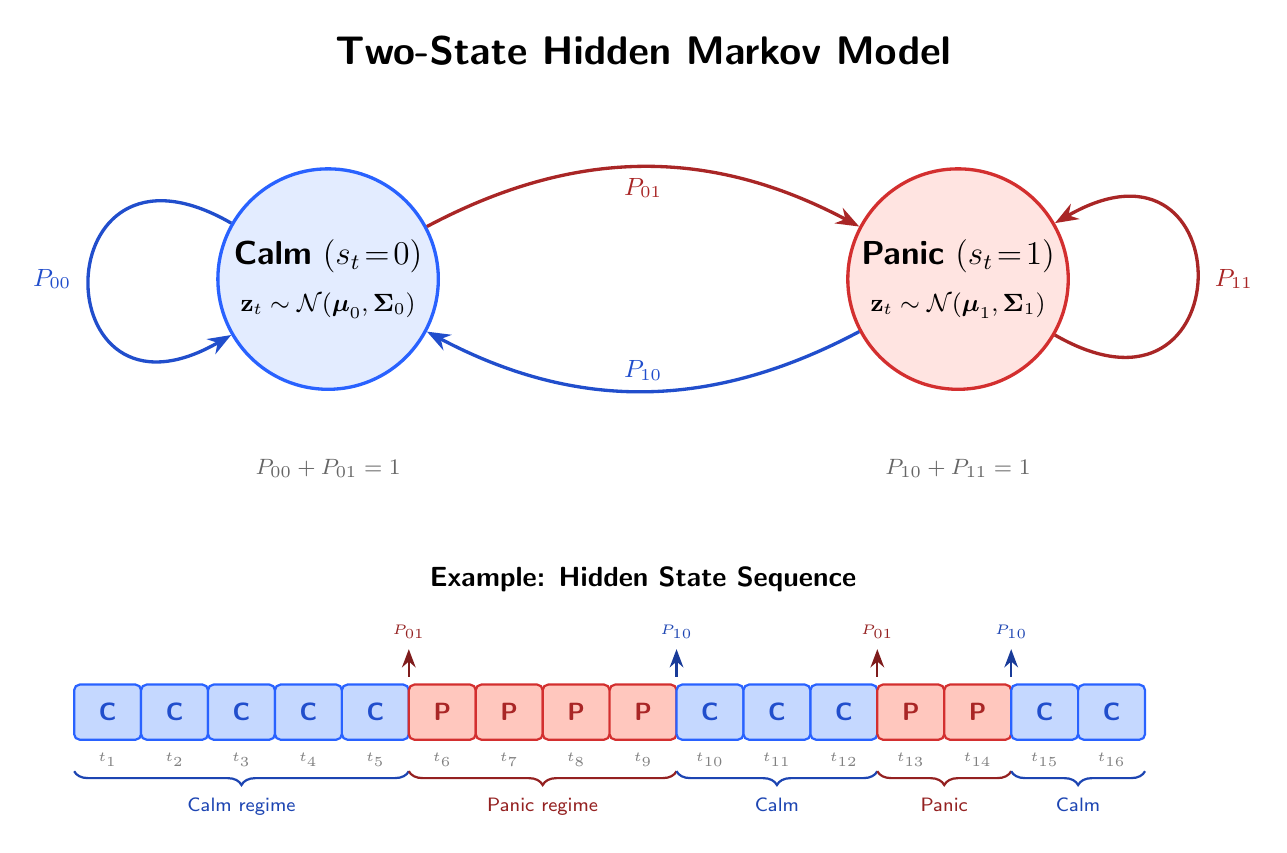
\begin{tikzpicture}[
    >=Stealth,
    every node/.style={font=\sffamily},
    state/.style={
        circle, draw, very thick, minimum size=2.8cm,
        inner sep=0pt, align=center, font=\sffamily\large
    },
    trans/.style={->, very thick, bend left=28},
    selflabel/.style={font=\sffamily\small, fill=white, inner sep=2pt}
]

%% ── States ──
\node[state, draw=calmblue, fill=calmfill] (calm) at (0,0) {
    \textbf{Calm} $(s_t\!=\!0)$\\[3pt]
    {\small $\mathbf{z}_t \sim \mathcal{N}(\boldsymbol{\mu}_0, \boldsymbol{\Sigma}_0)$}
};
\node[state, draw=panicred, fill=panicfill] (panic) at (8,0) {
    \textbf{Panic} $(s_t\!=\!1)$\\[3pt]
    {\small $\mathbf{z}_t \sim \mathcal{N}(\boldsymbol{\mu}_1, \boldsymbol{\Sigma}_1)$}
};

%% ── Transitions ──
\draw[trans, panicred!80!black] (calm) to node[below, pos=0.5, font=\sffamily\small] {$P_{01}$} (panic);
\draw[trans, calmblue!80!black] (panic) to node[above, pos=0.5, font=\sffamily\small] {$P_{10}$} (calm);

%% ── Self-loops ──
\draw[->, very thick, calmblue!80!black]
    (calm) edge [out=150, in=210, looseness=5]
    node[selflabel, left=4pt] {$P_{00}$} (calm);
\draw[->, very thick, panicred!80!black]
    (panic) edge [out=330, in=30, looseness=5]
    node[selflabel, right=4pt] {$P_{11}$} (panic);

%% ── Constraints ──
\node[font=\sffamily\footnotesize, text=black!60] at (0, -2.4) {$P_{00} + P_{01} = 1$};
\node[font=\sffamily\footnotesize, text=black!60] at (8, -2.4) {$P_{10} + P_{11} = 1$};

%% ── Title ──
\node[font=\sffamily\bfseries\Large, above] at (4, 2.6) {Two-State Hidden Markov Model};

%% ═══════════════════════════════════════════════
%% ── Example state sequence ──
%% ═══════════════════════════════════════════════
\def\seqy{-5.5}
\def\bw{0.85}
\def\bh{0.7}

\node[font=\sffamily\bfseries, above] at (4, \seqy + 1.4) {Example: Hidden State Sequence};

%% Calm: t1--t5
\foreach \i in {0,1,2,3,4} {
    \pgfmathsetmacro{\x}{-2.8 + \i * \bw}
    \fill[seqcalm, draw=calmblue, thick, rounded corners=2pt]
        (\x - \bw/2, \seqy - \bh/2) rectangle (\x + \bw/2, \seqy + \bh/2);
    \node[font=\sffamily\small\bfseries, text=calmblue!80!black] at (\x, \seqy) {C};
    \pgfmathtruncatemacro{\ti}{\i + 1}
    \node[font=\sffamily\tiny, text=black!50, below] at (\x, \seqy - \bh/2 - 0.05) {$t_{\ti}$};
}
%% Panic: t6--t9
\foreach \i in {5,6,7,8} {
    \pgfmathsetmacro{\x}{-2.8 + \i * \bw}
    \fill[seqpanic, draw=panicred, thick, rounded corners=2pt]
        (\x - \bw/2, \seqy - \bh/2) rectangle (\x + \bw/2, \seqy + \bh/2);
    \node[font=\sffamily\small\bfseries, text=panicred!80!black] at (\x, \seqy) {P};
    \pgfmathtruncatemacro{\ti}{\i + 1}
    \node[font=\sffamily\tiny, text=black!50, below] at (\x, \seqy - \bh/2 - 0.05) {$t_{\ti}$};
}
%% Calm: t10--t12
\foreach \i in {9,10,11} {
    \pgfmathsetmacro{\x}{-2.8 + \i * \bw}
    \fill[seqcalm, draw=calmblue, thick, rounded corners=2pt]
        (\x - \bw/2, \seqy - \bh/2) rectangle (\x + \bw/2, \seqy + \bh/2);
    \node[font=\sffamily\small\bfseries, text=calmblue!80!black] at (\x, \seqy) {C};
    \pgfmathtruncatemacro{\ti}{\i + 1}
    \node[font=\sffamily\tiny, text=black!50, below] at (\x, \seqy - \bh/2 - 0.05) {$t_{\ti}$};
}
%% Panic: t13--t14
\foreach \i in {12,13} {
    \pgfmathsetmacro{\x}{-2.8 + \i * \bw}
    \fill[seqpanic, draw=panicred, thick, rounded corners=2pt]
        (\x - \bw/2, \seqy - \bh/2) rectangle (\x + \bw/2, \seqy + \bh/2);
    \node[font=\sffamily\small\bfseries, text=panicred!80!black] at (\x, \seqy) {P};
    \pgfmathtruncatemacro{\ti}{\i + 1}
    \node[font=\sffamily\tiny, text=black!50, below] at (\x, \seqy - \bh/2 - 0.05) {$t_{\ti}$};
}
%% Calm: t15--t16
\foreach \i in {14,15} {
    \pgfmathsetmacro{\x}{-2.8 + \i * \bw}
    \fill[seqcalm, draw=calmblue, thick, rounded corners=2pt]
        (\x - \bw/2, \seqy - \bh/2) rectangle (\x + \bw/2, \seqy + \bh/2);
    \node[font=\sffamily\small\bfseries, text=calmblue!80!black] at (\x, \seqy) {C};
    \pgfmathtruncatemacro{\ti}{\i + 1}
    \node[font=\sffamily\tiny, text=black!50, below] at (\x, \seqy - \bh/2 - 0.05) {$t_{\ti}$};
}

%% ── Braces ──
\pgfmathsetmacro{\xa}{-2.8 + 0*\bw - \bw/2}
\pgfmathsetmacro{\xb}{-2.8 + 4*\bw + \bw/2}
\draw[decorate, decoration={brace, amplitude=5pt, mirror}, thick, calmblue!70!black]
    (\xa, \seqy - \bh/2 - 0.4) -- (\xb, \seqy - \bh/2 - 0.4)
    node[midway, below=6pt, font=\sffamily\scriptsize, text=calmblue!70!black] {Calm regime};

\pgfmathsetmacro{\xa}{-2.8 + 5*\bw - \bw/2}
\pgfmathsetmacro{\xb}{-2.8 + 8*\bw + \bw/2}
\draw[decorate, decoration={brace, amplitude=5pt, mirror}, thick, panicred!70!black]
    (\xa, \seqy - \bh/2 - 0.4) -- (\xb, \seqy - \bh/2 - 0.4)
    node[midway, below=6pt, font=\sffamily\scriptsize, text=panicred!70!black] {Panic regime};

\pgfmathsetmacro{\xa}{-2.8 + 9*\bw - \bw/2}
\pgfmathsetmacro{\xb}{-2.8 + 11*\bw + \bw/2}
\draw[decorate, decoration={brace, amplitude=5pt, mirror}, thick, calmblue!70!black]
    (\xa, \seqy - \bh/2 - 0.4) -- (\xb, \seqy - \bh/2 - 0.4)
    node[midway, below=6pt, font=\sffamily\scriptsize, text=calmblue!70!black] {Calm};

\pgfmathsetmacro{\xa}{-2.8 + 12*\bw - \bw/2}
\pgfmathsetmacro{\xb}{-2.8 + 13*\bw + \bw/2}
\draw[decorate, decoration={brace, amplitude=5pt, mirror}, thick, panicred!70!black]
    (\xa, \seqy - \bh/2 - 0.4) -- (\xb, \seqy - \bh/2 - 0.4)
    node[midway, below=6pt, font=\sffamily\scriptsize, text=panicred!70!black] {Panic};

\pgfmathsetmacro{\xa}{-2.8 + 14*\bw - \bw/2}
\pgfmathsetmacro{\xb}{-2.8 + 15*\bw + \bw/2}
\draw[decorate, decoration={brace, amplitude=5pt, mirror}, thick, calmblue!70!black]
    (\xa, \seqy - \bh/2 - 0.4) -- (\xb, \seqy - \bh/2 - 0.4)
    node[midway, below=6pt, font=\sffamily\scriptsize, text=calmblue!70!black] {Calm};

%% ── Transition markers ──
\pgfmathsetmacro{\xarr}{-2.8 + 4.5*\bw}
\draw[->, thick, panicred!60!black] (\xarr, \seqy + \bh/2 + 0.1) -- (\xarr, \seqy + \bh/2 + 0.45)
    node[above, font=\sffamily\tiny, text=panicred!70!black] {$P_{01}$};

\pgfmathsetmacro{\xarr}{-2.8 + 8.5*\bw}
\draw[->, thick, calmblue!60!black] (\xarr, \seqy + \bh/2 + 0.1) -- (\xarr, \seqy + \bh/2 + 0.45)
    node[above, font=\sffamily\tiny, text=calmblue!70!black] {$P_{10}$};

\pgfmathsetmacro{\xarr}{-2.8 + 11.5*\bw}
\draw[->, thick, panicred!60!black] (\xarr, \seqy + \bh/2 + 0.1) -- (\xarr, \seqy + \bh/2 + 0.45)
    node[above, font=\sffamily\tiny, text=panicred!70!black] {$P_{01}$};

\pgfmathsetmacro{\xarr}{-2.8 + 13.5*\bw}
\draw[->, thick, calmblue!60!black] (\xarr, \seqy + \bh/2 + 0.1) -- (\xarr, \seqy + \bh/2 + 0.45)
    node[above, font=\sffamily\tiny, text=calmblue!70!black] {$P_{10}$};

\end{tikzpicture}
\end{document}
